% -*- root: ../thesis.tex -*-

\chapter[Introduction]{Introduction}
\label{ch:intro}
\label{sec:intro:abs}

% \section{From actor \emph{modelling} to actor \emph{programming}}

Object-oriented programming~\cite{booch1982object,meyer1988object} has been of one the dominant paradigms for software engineering.
Object orientation provides principles for abstraction and encapsulation.
Abstraction is accomplished by high-level concepts of interfaces, classes, and objects (class instances).
Encapsulation provides means to hide implementation details of objects such as their internal state.
SIMULA 67~\cite{Dahl:1968:simula} introduced notions of classes, subclasses, and virtual procedures.
In the main block of a program, objects are created, then their procedures are called.
One object interacts with another object using the notion of a method.
Method invocations are \emph{blocking}; i.e. the caller object waits until it receives the result of the method call from the callee object.
This model of interaction was not the intention of the pioneers of the paradigm:
object interactions were meant to be \emph{messages} among objects and objects behaved as autonomous entities possibly on remote locations on a network; Alan Kay clarified later~\cite{alank1,alank2}. 
On the contrary, almost all the object-oriented languages at hand have followed the blocking and synchronous model of messaging. 
Object-oriented programming has inspired another paradigm: the actor model.

One of the fundamental elements of the actor model~\cite{actors:agha,agha97} is \emph{asynchronous} message passing.
In that approach, interactions between objects are modeled as non-blocking messages.
One object, the sender, communicates a message to the other object, the receiver.
In contrast with abstractions provided by object orientation, a message is not bound to any interface in the actor model.
At the receiver side, a message is matched with possible patterns and when a match is found, the message is processed by the receiver. 
Actor model features location transparency; i.e. the physical location of objects is not visible to other objects.
A system is composed of objects that communicate through messages.

A considerable amount of research has been carried out to combine object-oriented programming with the actor model~\cite{philippsen2000survey}. 
Language extensions, libraries, and even new programming languages are the  outcomes of such research.
For example, \cite{actor_frameworks_jvm:agha} presents a comparative analysis of such research for Java and JVM languages.

Multicore and distributed computing raised a new challenge: combining object orientation, the actor model, and \emph{concurrency}.
Concurrency motivates utilizing computational power to make programs run faster.
One goal has been to combine concurrency with object-oriented programming.
However, due to an exponential number of interleavings, concurrency makes it harder to verify programs in terms of correctness of runtime behavior~\cite{Herlihy:1990:linear,johnsen:history,agha:predictive:safety}. 
% Concurrency brings about two aspects in relation to object orientation:
% \emph{communication} and \emph{execution}.
Concurrency has different forms in different paradigms.

\paragraph*{Existing Concurrency Models}
In a concurrent setting, coroutines~\cite{conway1963design,taocp:knuth} enable interactions with collaborative pre-emption:
a coroutine has no \emph{return} statement, but it may explicitly \emph{yield}
to another coroutine (transfer control of the execution).
The yield relation is symmetric. 
Creating an instance of a coroutine spawns a new process with its own state.
A coroutine allows multiple entry points for suspending and resuming execution at explicitly specified locations.
The explicit interleaving points supports a compositional understanding of the code~\cite{DBLP:journals/cacm/Hoare74}.
coroutines are not originally established in the object-oriented paradigm.
Object orientation is based on caller-callee interaction, which is asymmetric:
the caller invokes a method in the callee and \emph{blocks} until the
corresponding \emph{return} occurs in the method of the callee.
Object orientation focuses on an object-view with caller-callee interaction and stack-based execution whereas coroutines focus on a process-view with flexible transfer of control.

In a concurrent setting with objects, multi-threading has been a common approach to provide an object-oriented concurrency model.
A thread holds a single stack of synchronous method calls.
Execution in a thread is sequential.
The stack has a starting location (i.e. start of invocation) and a finish location (i.e. the return point).
Future values can be used to hold the eventual return value of a method at the call site~\cite{DBLP:books/daglib/0092230,de2007complete}.
In a caller-callee setting, an object calls methods from other objects.
If multiple threads execute simultaneously in an object, their instructions are
interleaved in an uncontrolled manner.
In coroutines, the points of interleaving are explicit (i.e. \emph{yield}) 
whereas multi-threading is based on implicit scheduling of method invocations.
Furthermore, interactions in both coroutines and multi-threading are blocking and synchronous.
In contrast, the actor model relies on asynchronous communication (which is non-blocking)
as one of its core elements.

In the actor model, all communication is asynchronous.
The unit of communication is a \emph{message}.
A queue of messages (the inbox) is utilized among actors in the system.
The notion of a message is not bound to a specific definition or object interface.
When an actor receives a message, it may use pattern matching techniques to extract the content of the message.
When the actor completes the processing of a message, it may decide to reply to the message by sending another message.
The actor model works based on run-to-completion style of execution.
While a message is processed, an actor cannot be pre-empted or intentionally yield to allow other actors in the system to make progress.
Integration of actor model and object orientation leads to the use of asynchronous method calls.

\paragraph*{Problem Statement and Approach}
The main challenge is to generate production code from an actor-based language which supports asynchronous method calls and coroutine-style execution.
We take Java~\cite{gosling2000java} as the target programming language because it is one of the mainstream languages~\cite{tiobe} and it offers a wide range of mature and production-ready libraries and frameworks to use. 

% A question naturally rises: how to bring coroutine-style execution (co-operative scheduling) to an object-oriented setting with asynchronous communication through messages bound to object interfaces in a programming language?
% This question is the main problem statement of this thesis; cf. Table~\ref{tbl:problem}.

% \begin{table}[h]
% \centering
% \begin{tabular}{lll}
%  & OOP & Actor Model 
% \\ \toprule 
% \emph{Abstraction} & Class/Object & Actor 
% \\ \midrule
% \emph{Communication} & Sync. Method Call & Async. Message 
% \\ \midrule
% \emph{Execution} & Blocking + Stack-based & Blocking 
% \\ \midrule
% \emph{Concurrency} & Multi-threading & Multi-threading + RTC
% \\ \bottomrule
% \end{tabular}
% \caption[Summarized aspects of problem statement]{
% Considering the different aspects, the problem statement of thesis focuses to combine abstraction from OOP with asynchronous messages from Actor model but in a bounded context.
% In addition, this thesis focuses to bring in co-operative scheduling into the context of object-oriented programming.
% }
% \label{tbl:problem}
% \end{table}

There exist actor-based executable modeling languages that support asynchronous method calls and coroutine style execution; e.g. Rebeca and ABS.
Modeling languages are used to \emph{model} software systems for understanding, analysis, and verification. 
Execution of models is restricted to simulation.
As such, they do not generate production-ready code intended to run industrial environments.

Rebeca~\cite{sirjani2002simulation,sirjani2004formal,sirjani2007rebeca} is a modeling language for reactive and concurrent systems. 
In Rebeca, a number of reactive objects (\emph{rebecs}) interact at runtime.
Each rebec has its own unique thread of control and an unbounded queue of messages.
Rebecs interactions are based on asynchronous message passing.
Each message is put in the unbounded queue of the
receiver rebec and specifies a unique method to be invoked when the message
is processed.
Rebeca uses run-to-completion execution and does not support future values.

ABS~\cite{johnsen2012abs,hahnlehjlssw11} is a modeling language for concurrent objects and distributed systems.
ABS uses asynchronous communication among objects.
A message in ABS is bound to a method invocation;
this defines the interface of the sent messages.
In addition, ABS supports future values in its asynchronous communication.
ABS introduces \bfjtt{release} semantics that is based on co-operative scheduling of objects; 
i.e. similar to that of \emph{yield} in coroutines~\cite{creol:broch:owe}.
The ABS semantics is completely formalized by a structural operational semantics~\cite{plotkin:sos,abs:2012}.
This allows ABS models to take advantage of a wide range of static and dynamic analysis techniques~\cite{DBLP:journals/sttt/WongBBGGHMS15,DBLP:conf/cade/DinBH15,DBLP:conf/ifm/GiachinoGLLW13,DBLP:conf/tacas/AlbertAFGGMPR14}.
% 
Co-operative scheduling in ABS has been additionally extended for real-time scheduling with priorities and time constraints~\cite{bjork2013:rtabs,johnsen2012modeling}.
All the above characteristics make the ABS language an attractive choice if it
can be used as a programming language at industrial and business scale.
ABS has mainly developed as a modeling language;
for example, ABS does not support common I/O API for files or network,
and it does not provide a standard library of data structures.

JSR 166~\cite{jsr166} introduced a new concurrency model~\cite{DBLP:conf/java/Lea00} in Java 1.5.
The concurrency model lays the grounds to support actor model with asynchronous method calls.
This gave rise to various research to support actor model on Java~\cite{actor_frameworks_jvm:agha} and further extend Java as a functional programming language~\cite{odersky1997pizza,henkel2003discovering,nystrom2003polyglot,bracha1998making}.
From an industrial perspective, the development of Java language from version 6 to version 8 experienced a slow pace that influenced the growth of businesses and justified alternatives.
Scala~\cite{odersky2004scala}, a dynamic, functional, and object-oriented language on JVM, rose to the challenge to fill the gap during the period between Java~7 and Java~8.
Java~8~\cite{jls8} released fundamental features such as lambda expressions that are essential for concurrency and functional programming.

One core challenge is how to create a mapping of coroutines to multi-threading in Java.
Supporting coroutines in Java can be mostly classified in two major categories.
One category relies on a \emph{modified} JVM platform (e.g. Da Vinci JVM) in the implementation of thread stack and state such as \cite{Stadler:2009:LCJ:1596655.1596679}, \cite{Stadler:2010:ECJ:1852761.1852765} and \cite{Liu:2006:II:1111320.1111063}.
The other category involves libraries such as Commons Javaflow\footnote{\url{http://commons.apache.org/sandbox/commons-javaflow/}} or Coroutines\footnote{\url{https://github.com/offbynull/coroutines}} that utilize byte-code modification~\cite{dahm1999byte} at runtime in JVM.
In this research, we did not intend to use any of the two above approaches.
Custom or modified JVM platform implementations are not mainstream and not officially supported by the Java team which jeopardizes portability.
To keep up with new versions of the Java language, research and development of a modified JVM requires explicit and periodic maintenance and upgrade effort.
Moreover, as byte-code modification changes the byte-code of a running program or inserts new byte-code into JVM at runtime, this complicates reasoning and correctness analysis/verification~\cite{leroy2001java,leroy2003java}.
We aim to rely only on the mainstream JVM platform released by the Java team at Oracle.
Moreover, we do not intend to use byte-code engineering used for instance in Encore~\cite{fernandez2015parallel}.

Another straightforward way to support coroutines in Java multi-threading is that since a thread owns a single stack, we can translate every invocation (entry point) in a coroutine to a new thread in Java~\cite{SchaferP10,schafer2010programming}. 
This naive approach unsurprisingly leads to a poor performance since threads are resource-intensive in Java and the number of threads is not scalable at runtime due to resource limitations in JVM when the number of objects increase (cf. Chapter~\ref{ch:p01:ch01}).
Therefore, it is reasonable to use a pool of threads (JSR-166~\cite{jsr166}) to direct the execution of all method invocations (messages). 
% To deploy a message onto a thread for execution, the message can be abstracted in a generic way.
We utilize Java~8 features (JSR 335~\cite{jsr335} and JSR 292~\cite{jsr292:invokedyn}) to model a message as a data structure expressed in a lambda expression (cf. Chapter~\ref{ch:p02:ch01}).

\section{Objectives and Architecture}
\label{sec:intro:arch:crit}

In this section, we present a high-level overview of design goals of our framework and its implementation. 

\paragraph{Polyglot Programming}
With the rise of distributed computing challenges, software engineering practice has turned to methods that combine multiple programming languages and models to complete a task. 
In this approach, different languages with different focus and abstractions contribute to the same problem statement in different layers. 
Polyglot programming essentially enables software practice to apply the \emph{right} language in the appropriate layer of a system.
Layers of a system require points of integration.
ABS is an attractive choice for the concurrency and distributed layers.
Therefore, ABS should be able to provide integration points to other layers.
The programmer develops models with ABS that \emph{partially} take advantage of features of another language e.g. Java.
This approach is also referred to as \emph{Foreign Function Interface}.

\begin{lstlisting}[float=h,language=Java,caption=Using Java in ABS,label=lst:abs:java]
java.util.List<String> params = new java.util.ArrayList<>();    // Java
myObj ! doSomething(params);                                    // ABS
\end{lstlisting}

Listing~\ref{lst:abs:java} shows a snippet of ABS code that uses \jtt{java.util.ArrayList} as a data structure.
Ideally in ABS, the programmer is able to directly use the libraries and API from Java.
This removes the necessity to redundantly repeat definition of common data structures and API at ABS.
Furthermore, this allows to take advantage of the already rich and mature library API of Java.

\paragraph{Scalability} 
In distributed systems, the number of massages delivered among objects in the 
environment is not predictable at runtime.
The goal is to ensure the actor system scales in performance with least 
influence from the number of asynchronous messages delivered in the system.
Due to support of co-operative scheduling for asynchronous messages, ABS is a fit for distributed systems.

\paragraph{Separation of Concerns} 
We approach ABS modeling and development with a component-based or modular 
software engineering practices.
The scope of the research spans a number of layers around ABS language:

\begin{itemize}
\item \emph{Compiling ABS to a target programming language}
One first objective is to compile an ABS model to a target programming language.
Target languages potentially include mainstream programming languages such as
Java, Erlang, Haskell, and Scala.
%Thus, the ABS programmer should be able to use an ABS compiler to compile
%their ABS models to the target languages.
We propose a new architecture for the ABS tool-set and engineering that enables
different programming languages to utilize the same architecture.
\item \emph{Using ABS concurrency as an API in an existing programming language}
The ABS language syntax and semantics are formalized precisely and rigorously by a structural operational semantics~\cite{johnsen2012abs}.
If a mapping from ABS to a programming API is provided, a programmer is able to
take advantage of ABS semantics without directly programming in ABS.
This enables industry users of mainstream languages to
model their systems in ABS semantics using the programming languages and
platforms they are already familiar with.
\item \emph{Modular Architecture of ABS Tools}
ABS language provides rigorous semantics to model concurrent
and distributed systems.
For practical reasons, it is important that the user (that can be a programmer, an analyst, or a researcher) 
has access to a tool-set and IDE that allows working with ABS 
models in a user-friendly way.
The ABS IDE and tool-set should be easy to reuse and extend.
\end{itemize}

The above objectives and design principles are realized by the modular architecture presented in 
Figure~\ref{fig:arch}.

\begin{figure}[t]
\centering
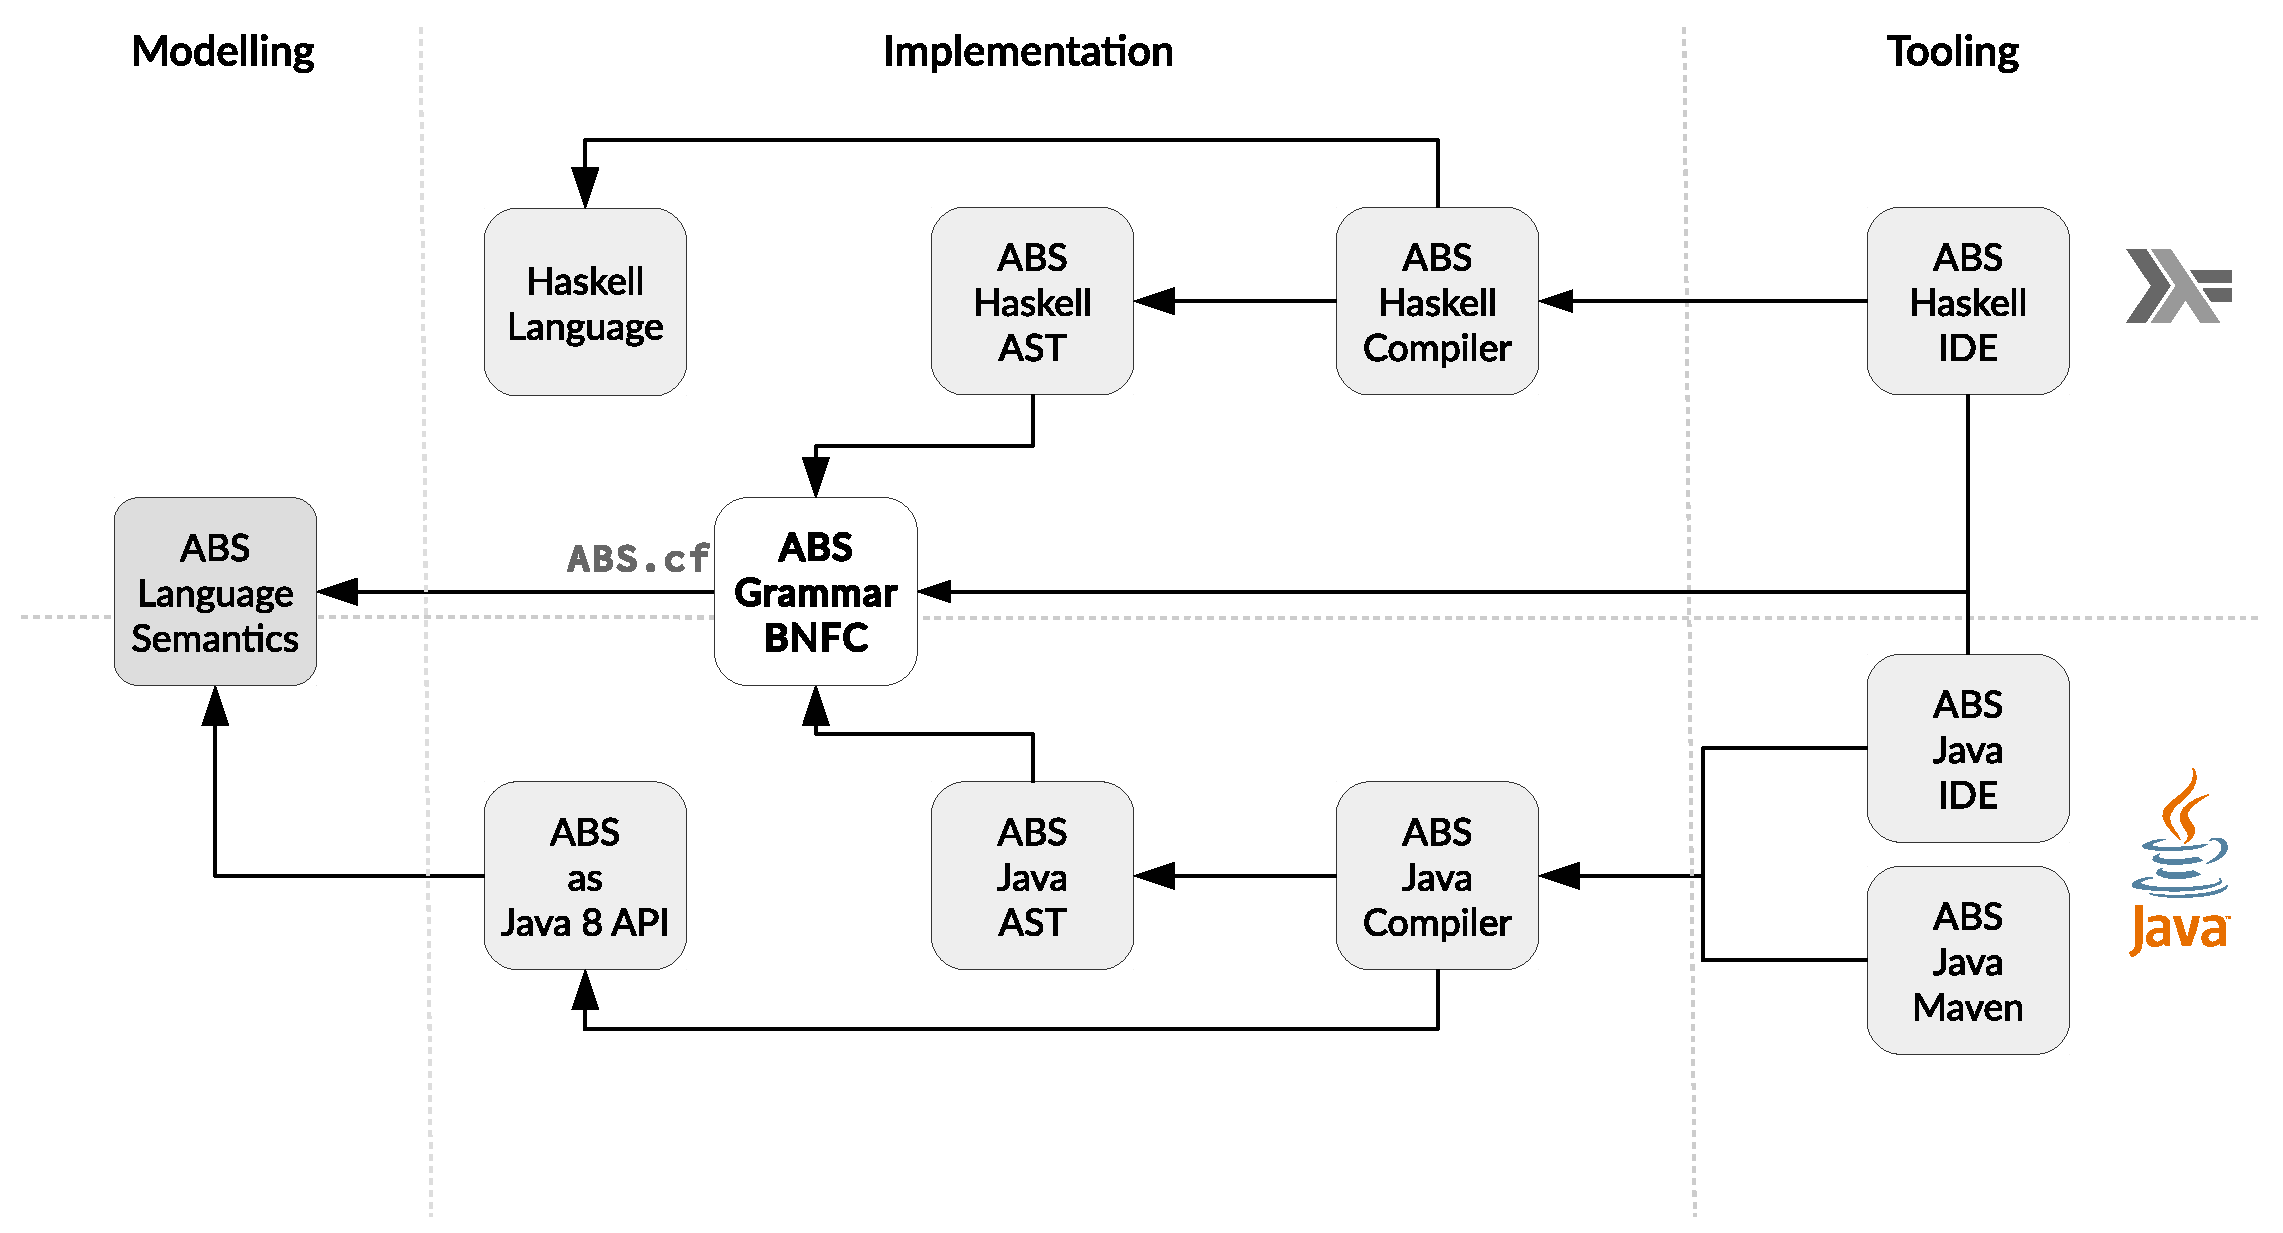
\includegraphics[scale=0.3]{../figs/Arch.eps}
\caption[General Architecture]{General Architecture of ABS API and Java Language Backend}
\label{fig:arch}
\end{figure}

\section{Literature Overview}
\label{sec:intro:rel}

We briefly discuss related work in the context of programming languages, actor model, and concurrency.
In the overview, we distinguish two levels; one is at the level of the programming languages and the other is for the external (third-party) libraries developed for programming languages.

\subsection{Programming Languages}
\label{sec:intro:proglangs}

In this section, we briefly provide an overview of the programming languages that have targeted similar problem statements.
Various programming languages, in the past decade, have emerged to provide an actor-based model of asynchronous message passing~\cite{philippsen2000survey}.
Table~\ref{tbl:actor:pl} presents different classes of actor model and concurrent model of programming.

\begin{description}
\item[First-Class Citizen]
Languages in which the actor model is by-design part of the syntax and 
semantics of the language.
Pony~\cite{ponylang,ClebschD13} targets high-performance 
computing using actor models and shared memory. 
Having the actor model as part of a language design simplifies formal verification.
\item[Implicit By Design]
Refers to languages that have no explicit notion of actors in their syntax or semantics, but do provide fundamental constructs for concurrency and asynchronous message passing.
Thus, it becomes an easy task in this kind of programming language to create an abstraction to support the actor model by coding.
% \item[External Library]
% Refers to the type of programming languages for which actor model support is provided by an external library.
\end{description}


\begin{table}[t]
\centering
\begin{tabular}{lll}
\textsfb{Language} & \textsfb{Abstraction} & \textsfb{Type} 
\\ \toprule
Erlang\cite{erlang:armstrong,erlang:actor} & Process & Implicit By Design 
\\ \midrule
Elixir\cite{elixir,elixir:actor} & Agent & Implicit By Design 
\\ \midrule
Haskell\cite{con_haskell:wiki} & forkIO \& MVars & Implicit By Design 
\\ \midrule
Go\cite{go:actor} & Goroutine & Implicit By Design 
\\ \midrule
Rust\cite{rust:2014,rust:actor} & Send \& Sync & Implicit By Design 
\\ \midrule
Scala\cite{haller09tcs} & Akka Actors
\footnote{Scala 2.11.0 adopts Akka as default actor model implementation: \url{http://docs.scala-lang.org/overviews/core/actors-migration-guide.html}}
& External Library 
\\ \midrule
Pony\cite{ponylang,ClebschD13} & actor & First-Class Citizen
\\ \bottomrule
\end{tabular}
\caption{Actor Model Support in Programming Languages}
\label{tbl:actor:pl}
\end{table}

\subsection{Frameworks and Libraries}
\label{sec:intro:libs}

Since programming languages faced challenges to provide the necessary syntax 
and semantics for actor model and concurrency at the level of the language, 
many libraries and frameworks aim to fill this gap 
Table~\ref{tbl:actor:libs} presents a summary.
We observe that the more the language itself is close to the actor model 
semantics, the less external libraries and frameworks target this gap. 
In the following, we briefly enumerate frameworks and libraries for JVM
\footnote{A more comprehensive list can be obtained at \cite{KarmaniSA09} and  \url{https://en.wikipedia.org/wiki/Actor_model\#Programming_with_Actors}}.

\begin{table}[t]
\centering
\begin{tabular}{lll}
\textsfb{Library} & \textsfb{Technique} & \textsfb{JVM Language} 
\\ \toprule
Killim\cite{srinivasan2008kilim,kilim} & Byte-Code Modification & Java 
\\ \midrule
Quasar\cite{quasar} & Byte-Code Modification, Java~8 & Clojure, Java 
\\ \midrule
Akka\cite{akka,scala:actors:ordersky} & Scala Byte-Code on JVM & Scala, Java 
\\ \bottomrule
\end{tabular}
\caption{Actor programming libraries in Java}
\label{tbl:actor:libs}
\end{table}

One of the main techniques used in libraries to deliver actor programming in 
JVM is byte-code engineering~\cite{dahm1999byte,bruneton2002asm,asm}.
Byte-code engineering modifies the generated byte-code for compiled classes in 
Java either during compilation or at runtime.
Although, this technique is commonly used and argued to provide better 
performance optimization~\cite{vallee1999soot}, it introduces challenges 
regarding the verification of the running 
byte-code~\cite{leroy2001java,leroy2003java}.

\section{Outline and Contributions}
\label{sec:intro:contribs}

The core contributions of this thesis target the intersection of object 
orientation, actor model, and concurrency.
We choose Java as the main programming language and as one of the mainstream 
object-oriented languages. 
We formalize a subset of Java and its concurrency API~\cite{jsr166} to 
facilitate formal verification and reasoning about it (cf. Chapter~\ref{ch:p01:ch02}).
We create an abstract mapping from a concurrent-object modeling language, 
ABS~\cite{johnsen2012abs}, to the programming semantics of concurrent Java (cf. Chapter~\ref{ch:p01:ch02}). 
We provide the formal semantics of the mapping and runtime properties of 
the concurrency layer including deadlines and scheduling policies (cf. Chapter~\ref{ch:p01:ch01}).
We provide an implementation of ABS concurrency layer as a Java API library 
and framework utilizing the latest language additions 
in Java 8~\cite{jsr335:lambda:translation} (cf. Chapter~\ref{ch:p02:ch01}).
We design and implement a runtime monitoring framework, JMSeq, to verify the
the correct ordering of execution of methods through code annotations in JVM (cf. Chapter~\ref{ch:p03:ch02}). 
In addition, we design a large-scale monitoring system as a real-world 
application; the monitoring system is built with ABS concurrent objects 
and formal semantics that leverages schedulability 
analysis to verify correctness of the monitors~\cite{fersman2007task} (cf. Chapter~\ref{ch:p03:ch01}).
Table~\ref{tbl:thesis} summarizes the structure of this text.

\begin{table}[t]
\centering
\begin{tabular}{p{7cm}p{3cm}p{3cm}}
\textsfb{Topic} & \textsfb{Part} & \textsfb{Chapter/Section}
\\ \toprule
{Formalization of the mapping from ABS to Java including the operational semantics and ABS co-operative scheduling in Java} & Programming Model (Part~\ref{p:model}) & Chapter~\ref{ch:p01:ch01} and \ref{ch:p01:ch02}
\\ \midrule
Design and implementation of ABS concurrency layer in Java & Implementation (Part~\ref{p:impl}) & Chapter~\ref{ch:p02:ch01} 
% and \ref{ch:p02:ch02}
\\ \midrule 
Monitoring method call sequences using annotations & Application (Part~\ref{p:app}) & Chapter~\ref{ch:p03:ch02}
\\ \midrule
Design and implementation of a massive-scale monitoring system based on ABS API in Java & Application (Part~\ref{p:app}) & Chapter~\ref{ch:p03:ch01}
\\ \bottomrule 
\end{tabular}
\caption{Thesis Organization}
\label{tbl:thesis}
\end{table}

\clearpage

In addition, Table~\ref{tbl:papers} summarizes the conference and journal 
publications as a result of this research:

\begin{table}[h]
\centering
\begin{tabular}{p{2cm}p{7cm}p{1cm}}
\textsfb{Topic} & \textsfb{Proceedings / Journal} & \textsfb{Year}   
\\ \toprule
Chapter~\ref{ch:p01:ch01} & ACM SAC 2012, Pages 1883--1888 & 2012 
\\ \midrule
Chapter~\ref{ch:p01:ch02} & COORD 2013, Pages 181--195 & 2013 
\\ \midrule
Chapter~\ref{ch:p02:ch01} & ISoLA 2014, Pages 37--53 & 2014 
\\ \midrule
Chapter~\ref{ch:p03:ch02} & Journal of Science of Computer Programming, 2014, Volume 94, Part 3, Pages 362--378 & 2014 
\\ \midrule
Chapter~\ref{ch:p03:ch01} & ESOCC 2015, Pages 125--140 & 2015
\\ \bottomrule
\end{tabular}
\caption{Actors At Work -- Conference and Journal Publications}
\label{tbl:papers}
\end{table}

All implementations of this thesis can be found at 

\begin{center}
\url{https://github.com/CrispOSS/abs-api-parent}
\end{center}

and the source of thesis can be found at

\begin{center}
\url{https://github.com/nobeh/thesis}
\end{center}
